\documentclass{ximera}
\title{Thevenin and Norton equivalent circuits}
\begin{document}
\begin{abstract}
This activity explains the theory of Thevenin and Norton equivalent circuits.
\end{abstract}

\maketitle

\section{Introduction}
There are many instances where we have have a complex circuit and would like to have a simple model for it.

In this exercise, we're going to work backwards: first we'll explore the behavior of the parts we know, and then we'll use that knowledge to describe systems we don't know about.

\section{Resistors}

\begin{exercise}
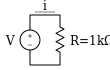
\includegraphics{figures/single_resistor.svg}

Write an equation for the current $i$ as a function of the voltage $V$.  Your solution should have the form $i = a \cdot V + b$, but a or b may be zero.

\begin{solution}
  \begin{hint}
    \begin{prompt}
      What is the y-intercept? \answer{0}
    \end{prompt}
  \end{hint}
  \begin{hint}
    Find the slope.  This will give you $a$.
    \begin{prompt}
      The slope is \answer{0.001} A/V.
    \end{prompt}
  \end{hint}
  
  $i = $ \answer{0.001V}
\end{solution}

Resistors have iV curves which are straight lines passing through the origin, and the slope is the inverse of the resistance.
\end{exercise}


\begin{exercise}
Write an equation:
\begin{solution}
  \begin{hint}
  \begin{prompt}
    What is the effective resistance, in Ohms, of the combined resistors? \answer{500}
  \end{prompt}
  \end{hint}

  $i = $ \answer{2x}
\end{solution}
\end{exercise}

\section{Current sources}
Now let's figure out current sources.
\begin{exercise}
Write an equation for the current $i$ as a function of the voltage $V$.  Again, your solution should have the form $i = a \cdot V + b$, but a or b may be zero.

\begin{solution}
  \begin{hint}
    Remember that a current source outputs the same current regardless of the voltage across it.
  \end{hint}
  \begin{hint}
  \begin{prompt}
    What is the y-intercept? \answer{0}
  \end{prompt}
  \end{hint}
 
  $i = $ \answer{1}
\end{solution}

\end{exercise}


% Every linear circuit produces a single line on the IV graph
% It makes sense, then, that we could represent every linear circuit using just a slope and an offset.

% What gives us slope?
% What gives us vertical offset?
% Horizontal offset?
% Why does the resistor have to be in series/parallel?

\end{document}
